\documentclass[11pt]{article}
\usepackage{multicol}
\setlength{\columnseprule}{1pt} % separation line between columns
\setlength{\parindent}{0pt} % paragraph indentation

\usepackage[top=2cm, bottom=2cm, left=2cm, right=2cm]{geometry}
\usepackage[T1]{fontenc}
\usepackage[utf8]{inputenc}
\usepackage[francais]{babel}
\usepackage{textcomp}

\usepackage{hyperref}
\hypersetup{
	colorlinks=true,       	% false: boxed links; true: colored links
	linkcolor=black,          	% color of internal links
	urlcolor=blue,           	% color of external links
	citecolor=blue
}

\usepackage{dashrule}
\usepackage{wrapfig}
\usepackage{graphicx}
\usepackage{enumitem}
\usepackage{wrapfig}
\usepackage{cancel} % diagonal strikeout
\usepackage[margin=1cm]{caption}
\setdescription{leftmargin=1cm,labelindent=0.5cm}

\usepackage{amsmath}
\usepackage{amssymb}
\usepackage{amsfonts}

\newcommand\mathd[0]{\mathrm{d}} 

\usepackage{blindtext}

% Colors
\usepackage[usenames,dvipsnames]{xcolor}
\definecolor{session_bg}{RGB}{25,25,25}
\definecolor{grey2}{rgb}{0.3,0.3,0.3}
\definecolor{dkgreen}{rgb}{0,0.6,0}
\definecolor{gray}{rgb}{0.5,0.5,0.5}
\definecolor{mauve}{rgb}{0.58,0,0.82}
\definecolor{blue}{rgb}{0,0,0.7}

% Colored frame
\usepackage{framed}
\definecolor{shadecolor}{rgb}{0.96,0.96,0.96}
\definecolor{TFFrameColor}{rgb}{0.96,0.96,0.96}
\definecolor{TFTitleColor}{rgb}{0.00,0.00,0.00}

% Redefine leftbar environment
\newlength{\leftbarwidth}
\setlength{\leftbarwidth}{1pt}
\newlength{\leftbarsep}
\setlength{\leftbarsep}{10pt}

\newcommand*{\leftbarcolorcmd}{\color{leftbarcolor}} % as a command to be more flexible
\colorlet{leftbarcolor}{gray}

\renewenvironment{leftbar}{%
    \def\FrameCommand{{\leftbarcolorcmd{\vrule width \leftbarwidth\relax\hspace {\leftbarsep}}}}%
    \MakeFramed {\advance \hsize -\width \FrameRestore }%
}{%
    \endMakeFramed
}

\usepackage{listings}
\lstloadlanguages{C,sh}
\lstdefinestyle{session}{
	numbers=left,	
	tabsize=4,
	frame=single, % cadre autour du code
	basicstyle=\small\ttfamily\color{white},
	numberstyle=\scriptsize\ttfamily,
	backgroundcolor=\color{session_bg},
	showstringspaces=false,
	keywordstyle=\color{OliveGreen},
	stringstyle=\color{BrickRed},
	commentstyle=\color{grey2}\it,
	stepnumber=1
}
\lstdefinestyle{C}{
    language=[ANSI]C,
	basicstyle=\scriptsize,
	numbers=left,                   % where to put the line-numbers
  	numberstyle=\tiny\color{gray},
	commentstyle=\color{dkgreen},
	frame=single,                   % adds a frame around the code
 	rulecolor=\color{black},
	emph={},
	emphstyle=\color{mauve},
	morekeywords={},
	keywordstyle={\color{blue}},
	showstringspaces=false
}

% Title page
\title{Création d'une interface graphique et interactive \\ pour jeux de rôles papier}
\author{
	Damien Martel \\ \href{mailto:damien.martel@edue.esiee.fr}{damien.martel@edu.esiee.fr} \and
	Bertrand Le Mée \\ \href{mailto:bertrand.lemee@edu.esiee.fr}{bertrand.lemee@edu.esiee.fr} \and
	Vincent Lindivat \\ \href{mailto:vincent.lindivat@edu.esiee.fr}{vincent.lindivat@edu.esiee.fr} \and
	Frédéric Nguyen \\ \href{mailto:frederic.nguyen@edu.esiee.fr}{frederic.nguyen@edu.esiee.fr}
}
\date{\today}

\begin{document}
\maketitle
\newpage
\hfill
\newpage
\tableofcontents
\newpage

\section{Introduction}

Le jeu de rôles (JdR) est un jeu qui regroupe plusieurs joueurs dans la même salle qui incarnent chacun un personnage pour jouer ensemble. Ils sont guidé par un Maître de Jeu qui orchestre le bon déroulement des sessions. Le jeu est accompagné de beaucoup de matériels tels que les dés, le plateau et les jetons. Cependant, un inconvénient se fait ressentir : il faut que toutes les personnes se trouvent dans la même pièce. Il n'est donc pas toujours facile pour les joueurs de se retrouver, particulièrement lorsqu'ils se situent loin géographiquement. \\

Ayant ces éléments à l'esprit, nous avons développé une interface graphique qui permet d'organiser des parties de jeu de rôles à distance sur réseau. Nous avons fait attention à ne pas dépayser les utilisateurs en conservant au mieux l'atmosphère du jeu de plateau habituel. \\

Ce projet est une opportunité pour nous de découvrir le travail de développement en équipe sur un projet de plus grande envergure que ce que nous avons réalisé jusqu'à maintenant.	

\section{Méthode agile SCRUM}

A l'occasion de ce projet, nous avons pu découvrir la méthode de développement
 agile SCRUM  et dans le même mouvement, appliquer cette méthode à la réalisation de notre projet.\\
 
Dans le cadre SCRUM, les trois entités suivantes se rassemblent autour du projet :

\begin{description}
	\item[Product Owner] \hfill \\
		Il définit les fonctionnalités du projet et décide de valider ou non les résultats. Il met en place les dates à respecter. Le Product Owner établit aussi le \textit{Backlog} avec le Scrum Master et l'équipe, mais il peut modifier un \textit{Sprint} si besoin.
	\item[Scrum Master] \hfill \\
		Il s'occupe de l'équipe de développement en veillant à ce que la méthode SCRUM soit bien appliquée. Il conseille son équipe et s'assure qu'elle progresse correctement. Il gère aussi les relations extérieures, particulièrement avec le Product Owner.
	\item[Equipe de développement] \hfill \\
		Généralement constituée de 5 à 10 personnes, l'équipe regroupe tout type de rôle. Une équipe travaille sur un \textit{Sprint} et est libre de s'organiser d'elle-même.
\end{description}

La progression du projet est basée sur un \textbf{Backlog}, faite par le Product Owner, le Scrum Master et l'équipe, qui est une liste ordonnée par priorité et complexité de temps de tâches à réaliser. Les priorités sont choisies par le Product Owner et peuvent être revues selon le courant des événements. \\

Durant le projet, le temps est divisé en séquence ayant une durée moyenne de 2 semaines, ces séquences sont appelées \textbf{Sprint}. Avant chaque Sprint, l'équipe choisit dans le Backlog l'ensemble des tâches qu'elle compte pouvoir réaliser. \\

Quotidiennement, une réunion d'une quinzaine de minutes \textbf{debout} se fait dans l'équipe afin de faire le point sur ce qui a été fait le jour précédent et ce qui va être fait le jour de la réunion. Lorsqu'un Sprint est terminé, le Product Owner, le Scrum Master et l'équipe se rassemblent pendant 30 minutes pour faire le point ce qui a marché et ce qui n'a pas marché afin de mieux préparer et agir lors du prochain Sprint. \\

N'étant qu'une équipe de 4 et le projet ne durant que 2 mois, nous avons dû réadapter la méthode. Nous nous sommes convenus de faire des Sprints de une semaine et travailler de façon très souple pendant les temps de travail.

\section{Manuel d'utilisation}

Cette application débute avec une boîte de dialogue qui laisse le choix entre deux rôles : Maître de Jeu (MJ) ou Joueur. Si "MJ" est choisi, l'application se met en tant que serveur pour accueillir les joueurs. Si "Joueur" est choisi, un assistant ce connexion apparaît pour choisir à quel serveur se connecter. \\

L'interface qui se présente comporte un Chat, un gestionnaire de tours et le lanceur de dés. Le Chat contient la liste des utilisateurs et permet aux joueurs et au MJ de communiquer. De plus, le chat possède des commandes qui s'introduisent par un /. Les commandes implémentées sont :

\begin{description}
	\item[/help] \hfill \\
		Affiche l'ensemble des autres commandes disponibles du chat avec les indications d'utilisation.
	\item[/nickname <pseudo>] \hfill \\
		Modifie le pseudo par celui qui suit la commande.
	\item[/roll <nombre de dés>d<valeur max du dé>] \hfill \\
		Roule un nombre de fois voulu du dé choisi. Peut s'utiliser en chuchotement.
	\item[/whisper <utilisateur> <message>] \hfill \\
		Envoie un message privé au joueur indiqué.
\end{description}

\begin{figure}[h!]
	\centering
	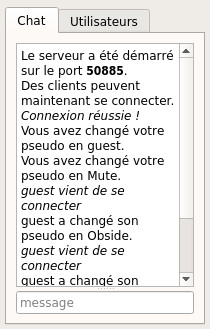
\includegraphics[scale=0.5]{img/chat_mj.jpg}
	\hspace{10 mm}
	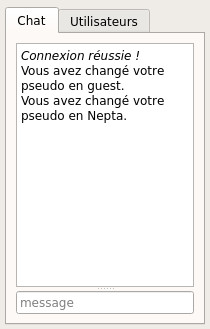
\includegraphics[scale=0.5]{img/chat_player.jpg}
	\caption{Chat MJ (à gauche) et chat Joueur (à droite)}
\end{figure}

Le Chat propose également une liste d'utilisateurs connectés. Un clic droit sur un ou plusieurs utilisateurs de cette liste affiche un menu contextuel donnant accès à des actions : Envoyer un message, et Lancer les dés.
La première action prépare un message privé à un ou plusieurs utilisateurs, la seconde lance les dés sélectionnés dans le lanceur de dés et envoie le résultat aux utilisateurs sélectionnés.


\begin{figure}[h!]
	\centering
	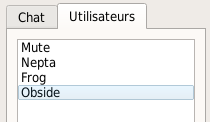
\includegraphics[scale=0.5]{img/chat_userlist_1.png}
	\hspace{10 mm}
	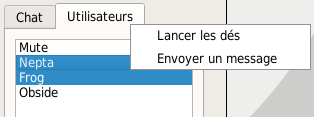
\includegraphics[scale=0.5]{img/chat_userlist_2.png}
	\caption{Liste d'utilisateurs (à gauche) et menu contextuel proposant des actions sur les utilisateurs sélectionnés (à droite)}
\end{figure}

Le lanceur de dés propose les dés les plus utilisés et permet de choisir pour chaque type de dé, le nombre de fois que celui-ci doit être lancé. Initialement, les compteurs sont à zéro. Pour augmenter le nombre de fois que l'on lance un dé, il faut appuyer sur le bouton correspondant ou utiliser la molette de la souris pour faire varier le nombre en étant sur le bouton. On peut ensuite décider de lancer les dés sur le chat (lancé public) ou de lancer les dés en privé si le MJ l'exige (lancé caché). Il est possible de réinitialiser tous les compteurs.

\begin{figure}[h!]
	\centering
	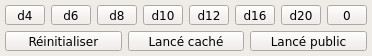
\includegraphics[scale=0.5]{img/dice_manager.jpg}
	\caption{Lanceur de dés}
\end{figure}

Le gestionnaire de tours est un outil qui permet au MJ de gérer ses combats. Il peut ajouter les joueurs ou personnages non joueurs (PNJ) en écrivant dans le champ de texte prévu à cet effet. Lorsque des utilisateurs se connectent, ils sont automatiquement ajoutés dans le gestionnaire de tour. Le MJ peut réordonner les tours à sa guise et dispose d'un certain nombre d'outils. Il peut ajouter des personnages comme dit précédemment, retirer un personnage à l'aide d'un bouton, déplacer les personnages dans le gestionnaire à la souris. Il dispose également de raccourcis clavier, par exemple les flèches du clavier permettent de naviguer entre les tours et de les réarranger.

\begin{figure}[h!]
	\centering
	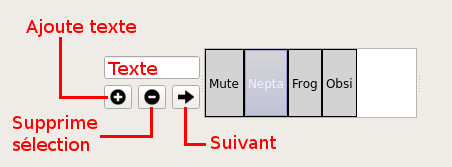
\includegraphics[scale=0.7]{img/turn_manager.jpg}
	\caption{Lanceur de dés}
\end{figure}

\section{Conclusion}

\end{document}